\subsection{Сцепление блоков шифртекста}
\selectlanguage{russian}

Режим сцепления блоков шифртекста (\langen{Cipher Block Chaining, CBC}, рис.~\ref{fig:CBC}) был описан в патенте компании IBM 1976 года.~\cite{Ehrsam:Meyer:Smith:Tuchman:1976} В этом режиме перед шифрованием текущего блока открытого текста предварительно производится его побитовое суммирование по модулю $2$ с предыдущим блоком зашифрованного текста, что и осуществляет <<сцепление>> блоков. Процедура шифрования имеет вид:
\[ \begin{array}{l}
    C_j = E_K(M_j \oplus C_{j-1}), ~ j = 1, 2, \dots, n,
\end{array} \]
где $C_0 = \textrm{IV}$ (сокр. от \langen{Initialization Vector}) -- блок, называемый вектором инициализации\index{вектор!инициализации}. Другое название -- синхропосылка\index{синхропосылка}.

\begin{figure}[bt]
	\centering
	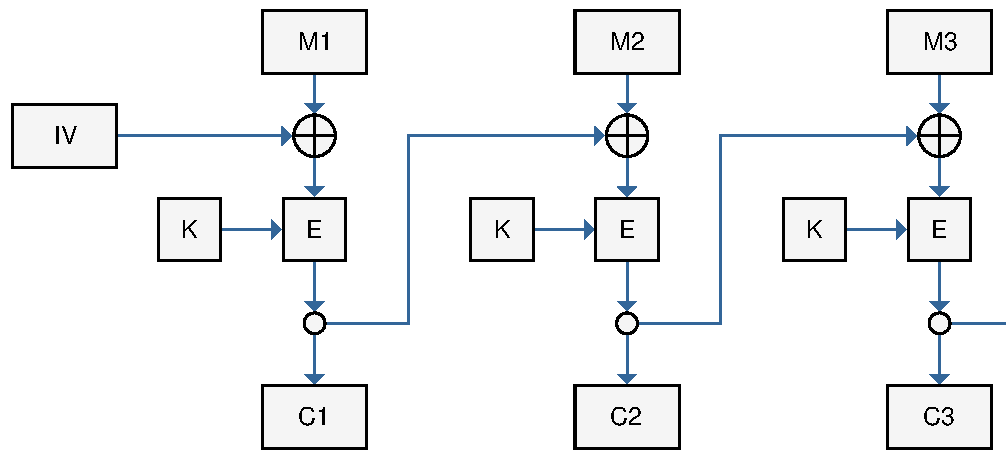
\includegraphics[width=1\textwidth]{pic/CBC}
	\caption{Режим сцепления блоков шифртекста}
	\label{fig:CBC}
\end{figure}

Благодаря сцеплению, \emph{одинаковым} блокам открытого текста соответствуют \emph{различные} шифрованные блоки. Это затрудняет криптоаналитику статистический анализ потока шифрованных блоков.

На приёмной стороне расшифрование осуществляется по правилу:
\[ \begin{array}{l}
    D_K(C_j) = M_j \oplus C_{j-1}, ~ j=1, 2, \dots, n,\\
    M_{j} = D_K(C_j) \oplus C_{j-1}.
\end{array} \]

Блок $C_0 = \textrm{IV}$ должен быть известен легальному получателю шифрованных сообщений. Обычно криптограф выбирает его случайно и вставляет на первое место в поток шифрованных блоков. Сначала передают блок $C_0$, а затем шифрованные блоки $C_1, C_2, \ldots, C_n$.

В разных пакетах блоки $C_0$ должны выбираться независимо. Если их выбрать одинаковыми, то возникают проблемы, аналогичные проблемам в режиме ECB. Например, часто первые нешифрованные блоки $M_1$ в разных пакетах бывают одинаковыми. Тогда одинаковыми будут и первые шифрованные блоки.

Однако случайный выбор векторов инициализации также имеет свои недостатки. Для выбора такого вектора необходим хороший генератор случайных чисел. Кроме того, каждый пакет удлиняется на один блок.

Для каждого сеанса передачи пакета нужны такие процедуры выбора $C_0$, которые известны криптографу и легальному пользователю. Одним из решений является использование так называемых \emph{одноразовых меток}. Каждому сеансу присваивается уникальное число. Его уникальность состоит в том, что оно используется только один раз и никогда не должно повторяться в других пакетах. В англоязычной научной литературе оно обозначается как \emph{Nonce}, то есть сокращение от <<Number used once>>\index{одноразовая метка}.

Обычно одноразовая метка состоит из номера сеанса и дополнительных данных, обеспечивающих уникальность. Например, при двустороннем обмене шифрованными сообщениями одноразовая метка может состоять из номера сеанса и индикатора направления передачи. Размер одноразовой метки должен быть равен размеру шифруемого блока. После определения одноразовой метки $\textrm{Nonce}$ вектор инициализации вычисляется в виде:
    \[ C_0 = \textrm{IV} = E_K(\textrm{Nonce}). \]

Этот вектор используется в данном сеансе для шифрования открытого текста в режиме CBC. Заметим, что блок $C_0$ передавать в сеансе необязательно, если приёмная сторона знает заранее дополнительные данные для одноразовой метки. Вместо этого достаточно вначале передать только номер сеанса в открытом виде. Принимающая сторона добавляет к нему дополнительные данные и вычисляет блок $C_0$, необходимый для расшифрования в режиме CBC. Это позволяет сократить издержки, связанные с удлинением пакета. Например, для шифра AES длина блока $C_0$ равна $16$ байтов. Если число сеансов ограничить величиной $2^{32}$ (вполне приемлемой для большинства приложений), то для передачи номера пакета понадобится только $4$ байта.

Преимущества:
\begin{itemize}
	\item отсутствие статистической зависимости блоков открытого текста и шифртекста;
\end{itemize}

Недостатки:
\begin{itemize}
	\item необходимость дополнения открытого текста до размера, кратного размеру блоку шифрования;
	\item невозможность параллельного шифрования (для следующего блока необходимо знать результат обработки предыдущего);
	\item ошибка передачи бита блока шифртекста приводит к ошибке расшифровки блока открытого текста целиком и к ошибке в одном бите следующего блока;
	\item не обеспечивает целостность.
\end{itemize}

Говоря о возможности восстановления после ошибок передачи, в режиме CBC при изменении одного бита блока шифртекста будет полностью некорректно расшифрован соответствующий блок отрытого текста, а также единственный бит \emph{следующего} блока открытого текста. Однако последующие блоки затронуты не будут. Поэтому данный режим относят к \emph{самовосстанавливающимся}.

Данный режим (как и большая часть остальных рассмотренных режимов) обеспечивает только конфиденциальность\index{конфиденциальность} передачи данных, но не целостность\index{целостность}. В модели активного злоумышленника, если последний предполагает о возможном содержимом первого блока открытого текста, а вектор инициализации передаётся в открытом виде по каналу связи, злоумышленник может подменить данные в векторе инициализации таким образом, чтобы сформировать нужное содержимое первого блока открытого текста. Такое изменение в режиме CBC не повлечёт других изменений и не приведёт к <<мусору>> в остальных блоках -- будет затронут только первый блок открытого текста. Изменение может не быть замечено получателем и привести к таким действиям получателя, которые ожидает злоумышленник, а не легальный отправитель.